\documentclass[tikz,border=4mm]{standalone}
\usepackage{pgfplots}
\pgfplotsset{compat=1.18}
\begin{document}
\pagecolor{white}
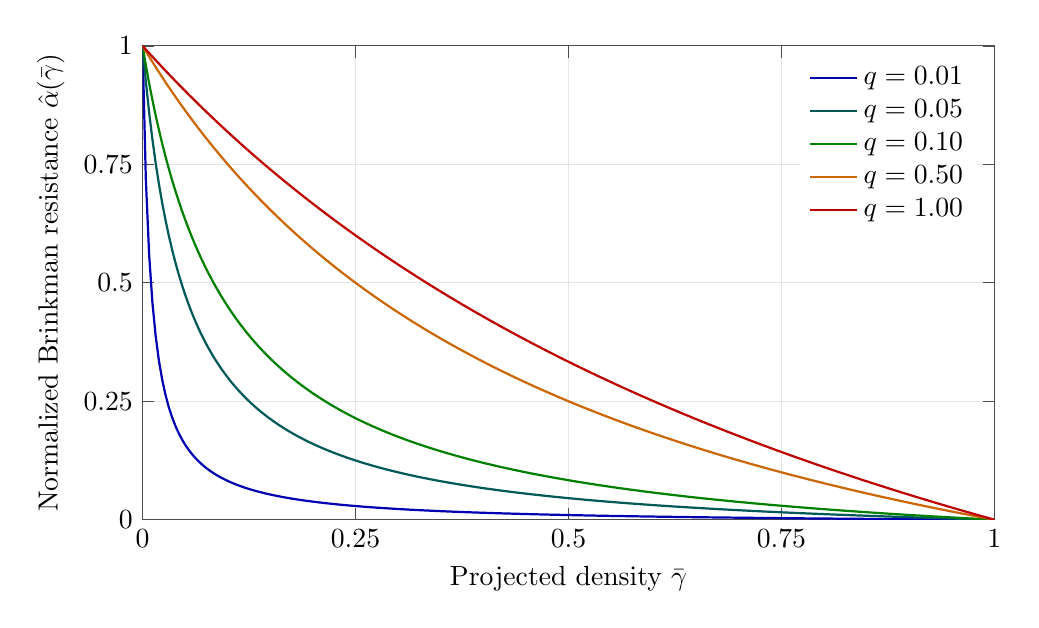
\begin{tikzpicture}
\begin{axis}[
	width=12.4cm,
	height=7.6cm,
	xmin=0, xmax=1,
	ymin=0, ymax=1,
	xlabel={Projected density $\bar{\gamma}$},
	ylabel={Normalized Brinkman resistance $\hat{\alpha}(\bar{\gamma})$},
	xtick={0,0.25,0.5,0.75,1},
	ytick={0,0.25,0.5,0.75,1},
	xticklabels={$0$,$0.25$,$0.5$,$0.75$,$1$},
	yticklabels={$0$,$0.25$,$0.5$,$0.75$,$1$},
	grid=both,
	major grid style={black!10},
	minor grid style={black!5},
	axis background/.style={fill=white},
	axis line style={black!70},
	tick style={black!70},
	legend cell align=left,
	legend style={draw=none, fill=white, fill opacity=0.92, text opacity=1, at={(0.98,0.98)}, anchor=north east}
]
\addplot[thick, blue!70!black, domain=0:1, samples=260] {1 - x*(1+0.01)/(x+0.01)};
\addlegendentry{$q=0.01$}
\addplot[thick, teal!70!black, domain=0:1, samples=260] {1 - x*(1+0.05)/(x+0.05)};
\addlegendentry{$q=0.05$}
\addplot[thick, green!50!black, domain=0:1, samples=260] {1 - x*(1+0.10)/(x+0.10)};
\addlegendentry{$q=0.10$}
\addplot[thick, orange!80!black, domain=0:1, samples=260] {1 - x*(1+0.50)/(x+0.50)};
\addlegendentry{$q=0.50$}
\addplot[thick, red!75!black, domain=0:1, samples=260] {1 - x*(1+1.00)/(x+1.00)};
\addlegendentry{$q=1.00$}
\end{axis}
\end{tikzpicture}
\end{document}
